% Generated by code/scripts/report_figures.py at 2026-11-03T07:57:50Z; do not edit.
% Inputs: artifacts/local/runs/pipeline-e2e-20261103T075711Z/run
\begin{figure}[t]
\centering
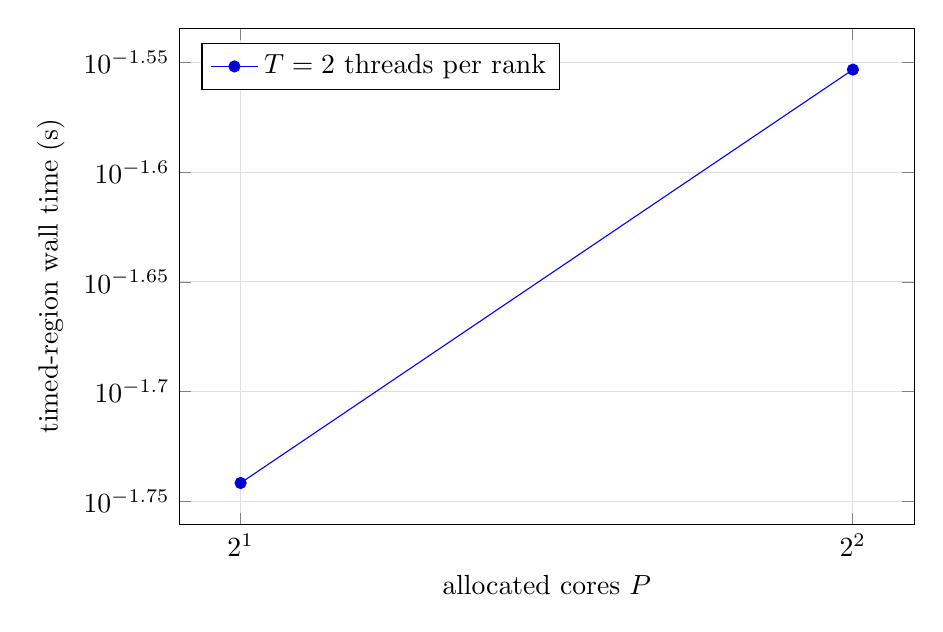
\begin{tikzpicture}
\begin{axis}[width=0.9\columnwidth, height=0.65\columnwidth, xlabel={allocated cores $P$}, ylabel={timed-region wall time (s)}, xmode=log, log basis x=2, ymode=log, legend pos=north west, legend cell align=left, grid=major, grid style={gray!25}]
\addplot+[mark=*] coordinates {(2,0.01812) (4,0.02797)};
\addlegendentry{$T=2$ threads per rank}
\end{axis}
\end{tikzpicture}
\caption{\textbf{LOCAL PIPELINE TEST, NOT A MEASUREMENT.} Weak-scaling runtime. $T=2$: $P_0=2$, $N_0=2000$, 1000 particles per core. Constant particles per core is not constant work per core.}
\label{fig:weak-runtime}
\end{figure}
